\documentclass[../DS08.tex]{subfiles}%
\graphicspath{{./figures/}}%

% \subimport{/home/nora/Documents/Enseignement/Prepa/bpep/exercices/DS/chimie_du_chrome/}{sujet.tex}%

\begin{document}%
\exercice[43]{Autour du chrome\ifcorrige{~\small\textit{(D'après Centrale TSI
			2007)}}}%

\enonce{
	\begin{tcn}[sidebyside, righthand ratio=.3](data){Données}
		Du grec khrôma ou du latin chroma (couleur).
		\smallbreak
		Il a été découvert par Louis Vauquelin en 1797. Il est présent dans la croûte
		terrestre ($0,03\%$), où on le trouve sous forme de chromite \ce{FeCr2O4}.
		%   On le trouve également dans le règne végétal dans la canne à sucre, la levure de
		% bière, les noix, les épices et dans le règne animal dans le foie et les
		% graisses.
		Il est utilisé dans le chromage des métaux, le tannage du cuir, la
		teinture de tissus, dans les matériaux d'enregistrement audio et vidéo (oxyde
		de chrome) ou encore la fabrication de pigments (le chromate de plomb est un
		pigment jaune et un oxyde de chrome est utilisé dans l'industrie du verre pour
		donner la couleur vert émeraude).
		%   Il est également employé pour faire des
		% alliages comme l'acier inoxydable ($70\%$ Fe, $20\%$ Cr, $10\%$ Ni). Plusieurs
		% de ses sels sont de puissants oxydants.
		\tcblower
		\begin{itemize}%
			\item $Z(\ce{Cr})=24$
			\item $K_e=10^{-14}$
			\item $K_{s_1}(\ce{Cr(OH)3})=10^{-31}$
			\item $K_{s_2}(\ce{Ag2CrO4})=10^{-12}$
		\end{itemize}%
	\end{tcn}
}%

% \subsection{Configurations électroniques}%
% \QR{%
% 	Énoncer la règle de Klechkowski. En déduire la configuration électronique du chrome dans son état fondamental en respectant cette règle. Préciser le nombre d'électrons de valence.
% }{%
% 	D'après la règle de Klechkowski, l'état fondamental d'un atome ou d'un ion monoatomique est obtenu en remplissant les sous-couches par ordre croissant énergétique soit par ordre croissant de $n+l$ et en cas d'égalité par ordre croissant de $n$.
%
% 	\ce{Cr}~: $1s^22s^22p^62s^23p^64s^23d^4$
%
% 	Le chrome a 6 électrons de valence.
% }%
%
% \QR{%
% 	En réalité, le chrome est une exception à la règle de Klechkowski. Donner alors la configuration électronique du chrome dans son état fondamental. Quelle est, en quelques mots, l'origine de cette exception à la règle de remplissage~?
% }{%
% 	On a un effet stabilisant lié à des sous-couches à moitié remplies.
%
% 	\ce{Cr}~: $1s^22s^22p^62s^23p^64s^13d^5$
% }%
%
% \QR{%
% 	Le chrome est-il un métal de transition~? Justifier la réponse.
% }{%
% 	Le chrome appartient au bloc $d$, c'est donc un métal de transition.
% }%
%
% \QR{%
% 	Donner la configuration électronique de l'ion \ce{Cr^{3+}}.
% }{%
% 	Ce sont les électrons de la sous-couche $4s$ qui sont arrachés en premier.
%
% 	\ce{Cr^{3+}}~: $1s^22s^22p^62s^23p^63d^3$
% }%

\subsection{Les ions en solution aqueuse}%
\enonce{%
	\noindent
	\begin{minipage}[c]{.55\linewidth}
		En solution aqueuse, le cation \ce{Cr^{3+}} (de couleur verte) donne avec les
		ions hydroxyde un précipité \ce{Cr(OH)_3} et un ion \ce{Cr(OH)_4^-}. En
		solution, la solubilité de l'hydroxyde peut s'écrire~:
		\[
			s = [\ce{Cr^{3+}}] + [\ce{Cr(OH)_4^-}]
		\]
		La courbe donnant la variation du logarithme décimal de la solubilité en
		fonction du pH est donnée sur la figure~\ref{fig:s}, pour une concentration
		totale $C_0$ en chrome III en solution.
	\end{minipage}
	\hfill
	\begin{minipage}[c]{.40\linewidth}
		\begin{center}
			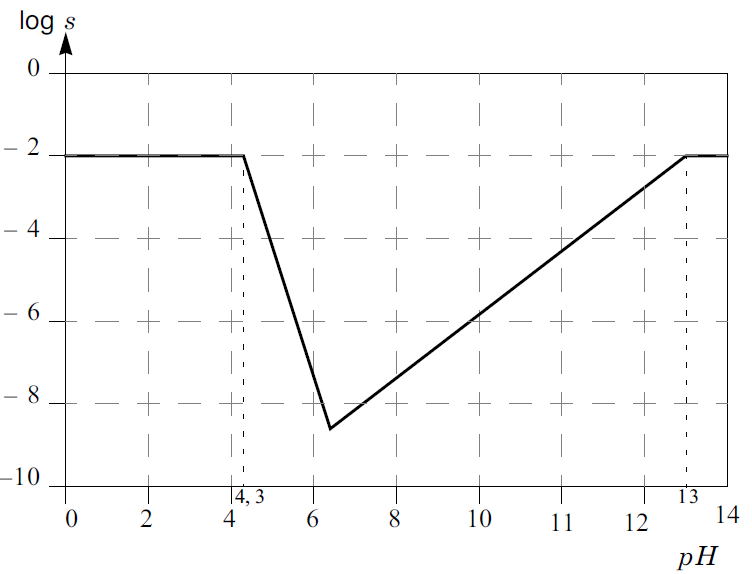
\includegraphics[width=\linewidth]{solubilite}
			\captionof{figure}{Influence du pH sur la solubilité des espèces du chrome.}
			\label{fig:s}
		\end{center}
	\end{minipage}
}%

\QR[2]{%
	Pourquoi peut-on parler pour \ce{Cr(OH)3} d'hydroxyde «~amphotère~»~?
}{%
	Un amphotère est une espèce à la fois acide et basique. Or, \ce{Cr(OH)3} est la
	base de \ce{Cr^{3+}} et l'acide de \ce{Cr(OH)_4^-}~:
	\begin{align*}
		\ce{Cr^{3+}_{\aqu} + 3H2O_{\liq} & \stm{=} Cr(OH)3_{\aqu} + 3H^+_{\aqu}}
		\\
		\ce{Cr(OH)3_{\aqu} + H2O_{\liq}  & \stm{=} {Cr(OH)_4}^-_{\aqu} + H^+_{\aqu}}
	\end{align*}
}%

\QR[3]{%
	Montrer que le graphe précédent permet de placer, sur un axe gradué en pH, les
	domaines de \ce{Cr(OH)_3}, \ce{Cr^{3+}} et de \ce{Cr(OH)_4^-}, puis tracer ce
	diagramme. S'agit-il de domaines de prédominance ou d'existence~?
}{%
	La solubilité est plus faible lorsque le solide existe \pt{1}, soit pour
	$\pH\in [4,3~; 13]$. Il s'agit d'un domaine d'existence.
	\begin{center}
		\includegraphics[scale=1]{predom_chrome}
	\end{center}
}%

\QR[2]{%
	Quelle est la valeur de $C_0$~?
}{%
	Pour $\pH<4,3$ (ou $\pH>13$), $s = C_0$ \pt{1}. On en déduit
	$\xul{C_0 \stm{=} \SI{1e-2}{\mole\cdot\liter^{-1}}}$.
}%

\QR[4]{%
	Définir le produit de solubilité de \ce{Cr(OH)3} puis retrouver sa valeur à
	partir des résultats précédents.
}{%
	$K_{s_1}$ est la constante d'équilibre de la réaction de dissolution~:
	\begin{gather*}
		\ce{Cr(OH)_{3(s)} \stm{=} Cr^{3+}_{\aqu} + 3HO^-_{\aqu}}
		\tag*{$K_{s,1}$}
	\end{gather*}
	À $\pH=4,3$, il y a début de précipitation de \ce{Cr(OH)3} \pt{1}. Le solide est
	alors présent en quantité infinitésimale, donc il y a équilibre de
	précipitation. De plus $[\ce{Cr^{3+}}] = C_0$ et $[\ce{HO-}]=
		\SI[parse-numbers=false]{10^{\num{-9.7}}}{\mole\cdot\liter^{-1}}$.
	\smallbreak
	D'après la loi d'action de masse évaluée en ce point
	\[
		\boxed{K_{s_1} \stm{=} \frac{[\ce{Cr^{3+}}]\ind{eq}\cdot
				[\ce{HO-}]\ind{eq}^3}{{c^\circ}^4}}
		\Ra
		\xul{K_{s_1} \stm{=} 10^{-31,1}}
	\]
	Cette valeur est cohérente avec celle de $10^{-31}$ donnée dans l'énoncé.
}%

\subsection{Précipitation avec les ions \ce{Ag+}}%

\enonce{%
	Les ions chromate donnent avec les ions argent \ce{Ag+} un précipité rouge de
	chromate d'argent \ce{Ag2CrO4}. On néglige dans cette question les propriétés
	basiques de l'ion chromate.
}%

\QR[6]{%
	Quelle est la solubilité $s_2$ du chromate d'argent dans l'eau pure~?
}{%
	On écrit la réaction de dissolution, et on effectue un tableau d'avancement en
	concentration, en notant $s_2$ la solubilité~:
	\begin{center}
		\def\rhgt{0.35}
		\centering
		\begin{tabularx}{.6\linewidth}{|l|c||YdYdY|}
			\hline
			\multicolumn{2}{|c||}{
				$\xmathstrut{\rhgt}$
			\textbf{Équation}}     &
			$\ce{Ag_2CrO4_{\sol}}$ & $=$              &
			$2\ce{Ag^+_{\aqu}}$    & $+$              &
			$\ce{{CrO_4}^{2-}_{\aqu}}$  \tikzmark{EP}   \\
			\hline
			$\xmathstrut{\rhgt}$
			Initial                & $x = 0$          &
			excès                  & \vline           &
			$0$                    & \vline           &
			$0$                                         \\
			\hline
			$\xmathstrut{\rhgt}$
			Final                  & $x_f = x_{\equ}$ &
			excès                  & \vline           &
			$2s_2V$                & \vline           &
			$s_2V$ \tikzmark{RP}                        \\
			\hline
		\end{tabularx}
	\end{center}
	\tikz[remember picture, overlay]
	\node[right=20pt of pic cs:EP] {\pt{1}+\pt{1}};
	\tikz[remember picture, overlay]
	\node[above right=3pt and 30pt of pic cs:RP] {\pt{1}};
	\begin{gather*}
		\beforetext{Loi d'action de masse}
		{K_{s_2}} \stm{=} \frac{s_2(2s_2)^2}{{c^\circ}^3}
		\Lra
		\boxed{s_2 \stm{=} c^\circ \left ( \cfrac{{K_{s_2}}}{4} \right )^{1/3}}
		\Ra \xul{s_2 \stm{=} \SI{6,3e-5}{\mole\cdot\liter^{-1}}}%
	\end{gather*}
}%

\QR[7]{%
Le produit de solubilité de \ce{AgCl} vaut $K_{s_3}=10^{-10}$. Quel est le
		précipité le plus soluble~?
	}{%
		On écrit la réaction de dissolution, et on effectue un tableau d'avancement en
		concentration, en notant $s_3$ la solubilité~:
		\begin{center}
			\def\rhgt{0.35}
			\centering
			\begin{tabularx}{.6\linewidth}{|l|c||YdYdY|}
				\hline
				\multicolumn{2}{|c||}{
					$\xmathstrut{\rhgt}$
				\textbf{Équation}}  &
				$\ce{AgCl_{\sol}}$  & $=$              &
				$2\ce{Ag^+_{\aqu}}$ & $+$              &
				$\ce{{Cl}^{-}_{\aqu}}$  \tikzmark{EP2}   \\
				\hline
				$\xmathstrut{\rhgt}$
				Initial             & $x = 0$          &
				excès               & \vline           &
				$0$                 & \vline           &
				$0$                                      \\
				\hline
				$\xmathstrut{\rhgt}$
				Final               & $x_f = x_{\equ}$ &
				excès               & \vline           &
				$s_3V$              & \vline           &
				$s_3V$ \tikzmark{RP2}                    \\
				\hline
			\end{tabularx}
		\end{center}
		\tikz[remember picture, overlay]
		\node[right=25pt of pic cs:EP2] {\pt{1}+\pt{1}};
		\tikz[remember picture, overlay]
		\node[above right=3pt and 30pt of pic cs:RP2] {\pt{1}};
		\begin{gather*}
			\beforetext{Loi d'action de masse}
			{K_{s_3}} \stm{=} \frac{s_3^2}{{c^\circ}^2}
			\Lra
			\boxed{s_3 \stm{=} c^\circ \sqrt{K_{s_2}}}
			\Ra \xul{s_3 \stm{=} \SI{1.0e-5}{\mole\cdot\liter^{-1}}}%
		\end{gather*}
		Comme $s_2>s_3$, on en déduit que \ce{Ag2CrO_{4}} est plus soluble \pt{1}
		que \ce{AgCl}.
	}%

\QR[5]{%
	Déduire des résultats précédents une méthode de dosage des ions chlorure.
	Décrire alors les principales étapes du dosage.
}{%
	On utilise l'ion chromate comme \textbf{indicateur coloré} \pt{1} de fin de
	réaction lors du dosage des ions chlorure par les ions argent (méthode de
	Mohr)~: on introduit \textbf{quelques gouttes} \pt{1} de chromate de
	potassium dans le bécher contenant la solution d'ions chlorure à doser~;
	cette solution est dosée par le \textbf{nitrate d'argent} \pt{1}. Il
	apparaît \textbf{d'abord le précipité blanc} de chlorure d'argent \pt{1}
	\ce{AgCl_{(s)}}, puis lorsque les ions chlorure ont disparu (ou du moins
	qu'il en reste une quantité négligeable devant la quantité initiale), il y a
	alors apparition du précipité rouge de chromate d'argent \ce{Ag2CrO_{4(s)}}
	\pt{1}.
}%

\subsection{Dosage}%
\enonce{%
	\noindent
	\begin{minipage}[c]{.60\linewidth}
		Les ions chromate (jaune) \ce{CrO_4^{2-}} et dichromate (orange)
		\ce{Cr2O_7^{2-}} donnent lieu à un équilibre acido-basique~:
		\begin{gather*}
			\ce{Cr2O_7^{2-} + 3H2O = 2CrO_4^{2-} + 2H3O+}
			\tag*{$K^\circ$}
		\end{gather*}
		On dose $V_1=\SI{100,0}{\milli\liter}$ d'une solution de dichromate de
		potassium à la concentration $C_1$ par une solution d'hydroxyde de sodium à
		la concentration $C_2=\SI{0,10}{\mole\cdot\liter^{-1}}$. L'allure de la
		courbe de dosage est donnée sur la figure~\ref{fig:titrage}.
	\end{minipage}
	\hfill
	\begin{minipage}[c]{.30\linewidth}
		\begin{center}
			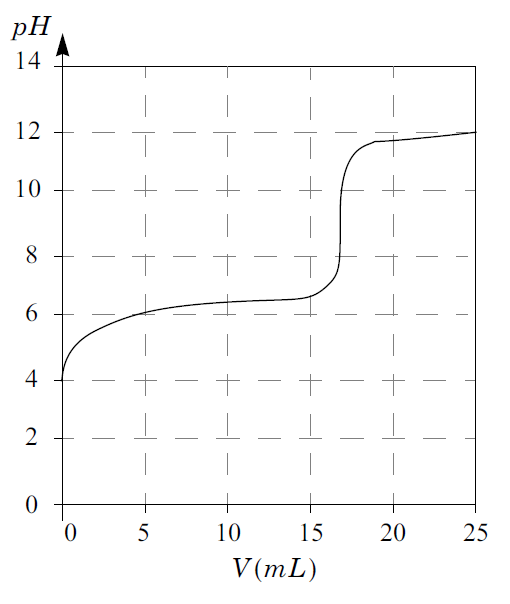
\includegraphics[width=\linewidth]{titrage}
			\captionof{figure}{Suivi pH-métrique du titrage.}
			\label{fig:titrage}
		\end{center}
	\end{minipage}
}%

\QR[2]{%
	Donner la structure de Lewis de l'ion dichromate, sachant que ce composé ne
	met en jeu que des liaisons \ce{Cr-O}.
}{%
	\begin{center}
		\chemfig{
		\chemabove{\charge{90=\|,180=\|,-90=\|}{O}}{\hspace{-0.5cm}\ominus}
		-Cr(
		=[2]\charge{45=\|,135=\|}{O}
		)(
		=[6]\charge{-135=\|,-45=\|}{O}
		)-\charge{90=\|,-90=\|}{O}
		-Cr(=[2]\charge{45=\|,135=\|}{O})
		(=[6]\charge{-135=\|,-45=\|}{O})
		-\chemabove{\charge{0=\|,90=\|,-90=\|}{O}}{\hspace{0.5cm}\ominus}}%
	\end{center}
}%

\QR[2]{%
	Quelles sont les électrodes utilisées pour le dosage~?
}{%
	C'est un titrage pH-métrique. Il faut donc une électrode combinée constituée
	d'une électrode de verre \pt{1} et d'une électrode de référence \pt{1} au
	calomel saturé par exemple.
}%

\QR[2]{%
Quelle est la réaction de dosage~?
}{%
C'est le titrage d'un acide faible par une base forte~:
\[
	\ce{{Cr_2O_7}^{2-}_{\aqu} + 2HO^-_{\aqu} \stm{\stm(un){=}} 2{CrO_4}^{2-}_{\aqu} + H2O_{\liq}}
\]
}%

\QR[3]{%
	Déduire de la courbe de dosage la valeur de $C_1$.
}{%
	On lit le volume à l'équivalence $V\ind{eq} = \SI{17}{\milli\liter}$ \pt{1}.

	À l'équivalence $C_1V_1 = \cfrac{C_2V\ind{eq}}{2}$, soit $\boxed{C_1 \stm{=}
			\cfrac{C_2V\ind{eq}}{2V_1}} \Ra \xul{C_1 \stm{=}
			\SI{8,5e-3}{\mole\cdot\liter^{-1}}}$.
}%

\QR[5]{%
	On lit le pH à la demi-équivalence $\pH_A=6,5$. Exprimer $K$ en fonction
	de $\pH_A$ et $C_1$. On négligera l'effet de la dilution au cours du
	titrage en considérant que le volume total de la solution vaut $V_1$ quel
	que soit le volume $V$ de soude versé. En déduire la valeur de $K^\circ$, ainsi
	que celle de la constante d'équilibre $K'$ de la réaction de titrage.
}{%
	\leavevmode\vspace*{-15pt}\relax
	\begin{gather*}
		\beforetext{Demi-équivalence}
		[\ce{CrO_4^{2-}}] = 2[\ce{Cr2O_7^{2-}}] = C_1 \pt{1}
		\\\beforetext{Loi d'action de masse}
		K^\circ \stm{=}
		\cfrac{[\ce{CrO_4^{2-}}]\ind{eq}^2[\ce{H3O+}]^2\ind{eq}}
		{[\ce{Cr2O_7^{2-}}]\ind{eq}{c^\circ}^3} = 2C_1 10^{-2{\pH_A}}
		\\\Lra
		\xul{K \stm{=} \num{1.7e-15}}
	\end{gather*}

	La constante d'équilibre de la réaction de titrage vaut alors $\xul{K' =
			\cfrac{K}{K_e^2} \stm{=} \num{1.7e13}\gg 1}$. Il s'agit bien d'une bonne réaction de
	titrage du point de vue de sa quantitativité. \pt{1}
}%

\end{document}%
